% This latex template was heavily modified by Dave Moffat 2020, 
% Originally derived from Edinburgh Napier's template. % https://www.overleaf.com/latex/templates/edinburgh-napier-coursework-report/gvrfkjrqhgcc
% #######################################
% ########### DEFINITIONS #############
% #######################################
\def\mytitle{Coursework Report Title}
\def\myauthor{My Name}
\def\mymodule{Music Fundamentals, Acoustics, and Perception (CAMT 401)}
\documentclass[11pt]{article}

\usepackage{a4wide}
\usepackage{graphicx}
\graphicspath{{./images/}}
\usepackage[colorlinks,linkcolor={black},citecolor={blue!80!black},urlcolor={blue!80!black}]{hyperref}
\usepackage[parfill]{parskip}
\usepackage{lmodern}
\renewcommand*\familydefault{\sfdefault}
\usepackage{watermark}
\usepackage{xcolor}
\usepackage{listings}
\usepackage{float}
\usepackage{titlesec}
\usepackage{amsmath}
\usepackage{natbib}
\usepackage{algorithm2e}

\titlespacing{\subsection}{0pt}{\parskip}{-3pt}
\titlespacing{\subsubsection}{0pt}{\parskip}{-\parskip}
\titlespacing{\paragraph}{0pt}{\parskip}{\parskip}
\newcommand{\figuremacro}[5]{
    \begin{figure}[#1]
        \centering
        \includegraphics[width=#5\columnwidth]{#2}
        \caption[#3]{\textbf{#3}#4}
        \label{fig:#2}
    \end{figure}
}

\lstset{
	escapeinside={/*@}{@*/}, 
	language=C++,
	basicstyle=\fontsize{8.5}{12}\selectfont,
	numbers=left,
	numbersep=2pt,
	xleftmargin=2pt,
	frame=tb,
    columns=fullflexible,
    showstringspaces=false,
    tabsize=4,
    keepspaces=true,
    showtabs=false,
    showspaces=false,
    backgroundcolor=\color{white}, 
    morekeywords={inline,public,
    class,private,protected,struct},
	captionpos=t,
	lineskip=-0.4em,
	aboveskip=10pt, 
	extendedchars=true, 
	breaklines=true,
	prebreak = \raisebox{0ex}[0ex][0ex]{\ensuremath{\hookleftarrow}},
	keywordstyle=\color[rgb]{0,0,1},
	commentstyle=\color[rgb]{0.133,0.545,0.133},
	stringstyle=\color[rgb]{0.627,0.126,0.941}
}

\thiswatermark{\centering \put(360,-70){
\includegraphics[width=0.33\textwidth]{logo}} }
\title{\mytitle \vspace{-1em}}
\author{\myauthor\hspace{1em}\\\mymodule}
\date{}
\hypersetup{pdfauthor=\myauthor,pdftitle=\mytitle}
\sloppy % Select the template to use

% #######################################
% ########### START FROM HERE ###########
% #######################################
\begin{document}
	\maketitle
	
	\section{Introduction}
	The purpose of this template, is to allow you to write and create reports for coursework on the Computing Audio and Music Technology BSc.
	
	\subsection{Referencing}
	You should cite References like this: \cite{Keshav} if you are talking about the author directly, as it will include the name, with the year in brackets. If you are adding a reference indirectly, then use \citep{Keshav}. The references are saved in an external .bib file, and will automatically be added to the bibliography at the end of this report once cited.
	
	
	\section{Formatting}
	Some common formatting you may need uses these commands for \textbf{Bold Text}, \textit{Italics}, and \underline{underlined}.
	\subsection{Line Breaks}
	Here is a line
	
	Here is a line followed by a double line break.
	This line is only one line break down from the above, Notice that latex can ignore this
	
	We can force a break \\ with the break operator.
	
	\subsection{Maths}
	Embedding Maths is what Latex was made to do. You can create inline equations with the dollar sign $x = \frac{y}{2} + z$. You can also produce full line equations with 
	
	$$\sqrt{-1} \, 2^3 \Sigma \pi $$
	
	Or you can make equations which are numbers, and can be referenced, using the begin and end equation block.
	
	\begin{equation}
		\label{Eq:filter}
		H(z) = \frac{1+2z^{-1}+z^{-2}}{1+\frac{1}{4}z^{-1}-\frac{3}{8}z^{-2}} = \frac{Y(z)}{X(z)}
	\end{equation}   
	
	\begin{equation}
		\label{Eq:infSum}
		\sum^\infty_{n=1} \frac{1}{n^2} = \frac{\pi^2}{6}
	\end{equation} 
	
	
	\section{Floats}
	Floats are the general concept of a block, whether an image, a table, some code or pseudocode. The idea in Latex is that Floats cannot be split over two pages, and need to remain whole, so the entire float needs to be placed in a nice location, and must be referenced and contain a caption.
	
	
	\subsection{Images}
	\begin{figure}[h]
		\centering
		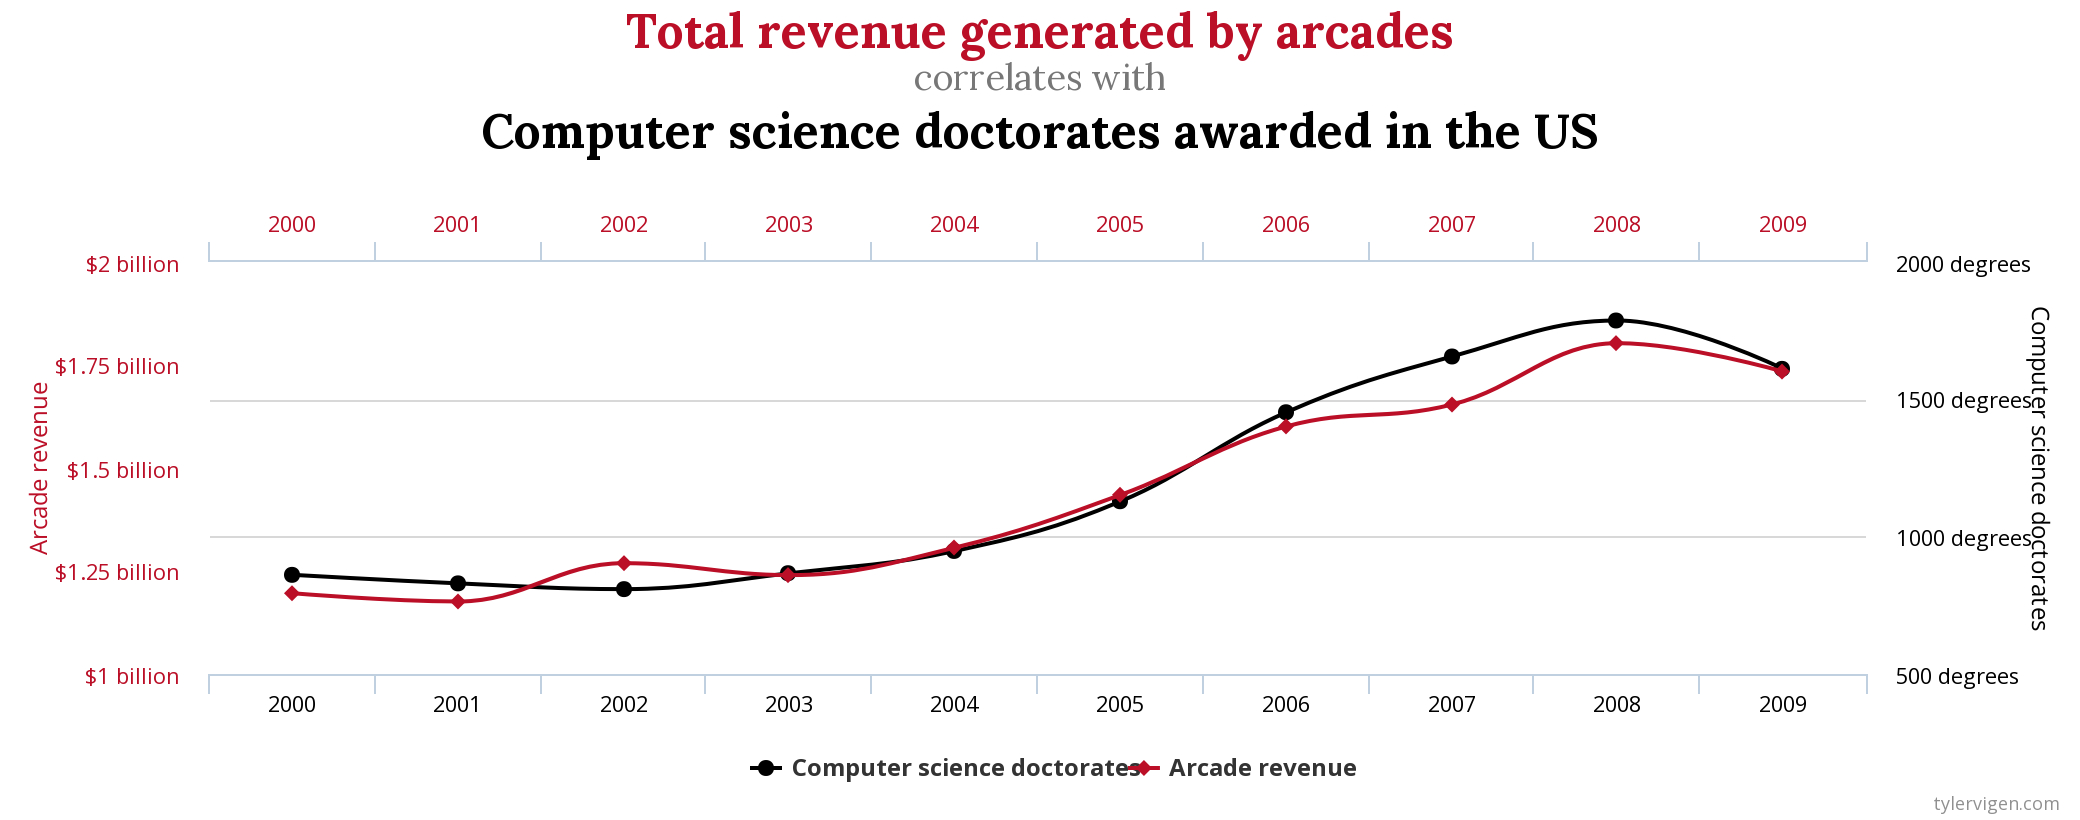
\includegraphics[width=\textwidth]{graph}
		\caption{Graph of correlation between arcade revenue and number of CS doctorates in the USA.}
		\label{fig:graph}
	\end{figure}
	
	\subsection{Tables}
	We can put a table in here \ref{tbl:example}
	

	\begin{table}[h]
		\centering
		\ \begin{tabular}{||c c c c||} 
		\hline
		Col1 & Col2 & Col2 & Col3 \\ [0.5ex] 
		\hline\hline
		1 & 6 & 87837 & 787 \\ 
		\hline
		2 & 7 & 78 & 5415 \\
		\hline
		3 & 545 & 778 & 7507 \\
		\hline
		4 & 545 & 18744 & 7560 \\
		\hline
		5 & 88 & 788 & 6344 \\ [1ex] 
		\hline
	\end{tabular}
	\caption{This is an example table}
	\label{tbl:example}
	\end{table}

 an outline of float arguments, is seen in Table \ref{tbl:floatPlacement}, taken from overleaf\footnote{\url{https://www.overleaf.com/learn/latex/Positioning_of_Figures}}
	\begin{table}[h]
		\centering
		\begin{tabular}{c | p{0.9\textwidth}} 
			specifier & resulting location \\
			\hline \hline
			h	& Place the float here, i.e., approximately at the same point it occurs in the source text (however, not exactly at the spot)\\
			t	& Position at the top of the page.\\
			b	& Position at the bottom of the page.\\
			p	& Put on a special page for floats only.\\
			!	& Override internal parameters LATEX uses for determining "good" float positions.\\
			H	& Places the float at precisely the location in the LATEX code. This is somewhat equivalent to h!, though some errors may arise if you have too many consecutive floats with [H].\\
		\end{tabular}
		\caption{Table of float placement arguments}
		\label{tbl:floatPlacement}
	\end{table}


	
	
	
	
	\subsection{Code Listing}
	You can load segments of code from a file, or embed them directly.
	
	\begin{lstlisting}[caption = Hello World! in c++, language=c++]
		#include <iostream>
		
		int main() {
			std::cout << "Hello, World!" << std::endl;
			std::cin.get();
			return 0;
		}
	\end{lstlisting}

	Or you can load code directly in from a file, instead of copying and pasting into a document.
	\lstinputlisting[caption = c++ listing from an input file, language=c++]{codeExample.cpp}
	
	
	\subsection{PseudoCode}
	\begin{algorithm}[h]
		\For{$i = 0$ \KwTo $100$}{
			print\_number = true\;
			\If{i is divisible by 3}{
				print "Fizz"\;
				print\_number = false\;
			}
			\If{i is divisible by 5}{
				print "Buzz"\;
				print\_number = false\;
			}
			\If{print\_number}{
				print i\;
			}
			print a newline\;
		}
		\caption{FizzBuzz}
	\end{algorithm}
	
	
	
	\section{Conclusion}	
	
	We have written a simple latex template with basic examples of how to perform the majority of tasks.
	``I always thought something was fundamentally wrong with the universe'' \citep{adams1995hitchhiker}
	
	
	\bibliographystyle{agsm}
	\bibliography{references}
	
\end{document}